%%%%%
%%
%% Onderzoeksverslag
%%
%% Version: v0.1
%% Authors: Iain Munro
%% Date: 18/02/2018
%%%%%

%Install packages using:
%sudo tlmgr install

% Available documentclass options:
%
%   <all `report` document class options, e.g.: `a5paper`>
%   withindex   - enables the index. New index entries can be added through `\index{my entry}`
%   glossary    - enables the glossary.
%   techreport  - typesets the thesis in the technical report format.
%   firstyr     - formats the document as a first-year report.
%   times       - uses the `Times` font.
%   backrefs    - add back references in the Bibliography section
%
% For more info see `README.md`
\documentclass[firstyr,a4paper,oneside]{cam-thesis}%withindex
\usepackage[dutch]{babel}
% Citations using numbers
\usepackage[numbers]{natbib}

\newcommand{\thesisTitle}{Allianz - Automatiseren Claim Process}

\usepackage[utf8]{inputenc}

%APA norm
\usepackage{babel} 
\usepackage{apalike}
\bibliographystyle{apalike}

%tables new lines
\usepackage{makecell}

%Set the title spacing correctly
\usepackage{titlesec}
\titlespacing{\chapter}{0pt}{0pt}{0pt}
\titlespacing{\section}{0pt}{0pt}{0pt}
\titlespacing{\subsection}{0pt}{0pt}{0pt}

%Om de pagina margins etc te debuggen
%\usepackage{showframe}

\usepackage{pgfgantt}
\usepackage{rotating}
\usepackage[graphicx]{realboxes}

%%%%%%%%%%%%%%%%%%%%%%%%%%%%%%%%%%%%%%%%%%%%%%%%%%%%%%%%%%%%%%%%%%%%%%%%%%%%%%%%
%% Style (Changing the visual style of chapter headings and stuff.)
%%
\RequirePackage{titlesec}
% [Fixes issue #34 (see https://github.com/cambridge/thesis/issues/34). Solution from: http://tex.stackexchange.com/questions/299969/titlesec-loss-of-section-numbering-with-the-new-update-2016-03-15
\RequirePackage{etoolbox}
\makeatletter
\patchcmd{\ttlh@hang}{\parindent\z@}{\parindent\z@\leavevmode}{}{}
\patchcmd{\ttlh@hang}{\noindent}{}{}{}
\makeatother
% end of issue #34 fix]
\newcommand{\PreContentTitleFormat}{\titleformat{\chapter}[display]{\scshape\Large}
{\Large\filleft\MakeUppercase{\chaptertitlename} \Huge\thechapter}
{1ex}
{}
[\vspace{1ex}\titlerule]}
\newcommand{\ContentTitleFormat}{\titleformat{\chapter}[display]{\scshape\huge}
{\Large\filleft\MakeUppercase{\chaptertitlename} \Huge\thechapter}
{1ex}
{\titlerule\vspace{1ex}\filright}
[\vspace{1ex}\titlerule]}
\newcommand{\PostContentTitleFormat}{\PreContentTitleFormat}
\PreContentTitleFormat

%Om dubbelen legen pagina's weg te halen.
\let\cleardoublepage=\clearpage

%%%%%%%%%%%%%%%%%%%%%%%%%%%%%%%%%%%%%%%%%%%%%%%%%%%%%%%%%%%%%%%%%%%%%%%%%%%%%%%%
%% Thesis meta-information
%%

%% The title of the thesis:
\title{Automatiseren Claim Process}

%% The full name of the author (e.g.: James Smith):
\author{Calum Iain Munro}

%% College affiliation:
\college{Software Development, ICA, VT}

%% College shield [optional]:
\collegeshield{CollegeShields/ICA}

%% Submission date [optional]:
\submissiondate{July, 2018}

%% You can redefine the submission notice [optional]:
\submissionnotice{
HBO bachelorscriptie:\\
\textbf{Versie: 1 (Draft)}\\
\textbf{Datum: \today}\\
\\~\\
\textbf{Gegevens opdrachtgever:}\\
Bedrijf:			HeadForward B.V.\\
Contactpersonen:	Dani\"el Siahaya\\
\\~\\
\textbf{Gegevens opleiding:}\\
Opleiding: HBO bachelor Informatica\\
School: Hogeschool van Arnhem en Nijmegen\\
Begeleider:	Misja Nabben\\
Assessor: Rein Harle\\
\\~\\
\textbf{Gegevens opdrachtnemer:}\\
Teamlid: Calum Iain Munro (549288)\\
}

%% Declaration date:
\date{Febuari, 2018}

%% PDF meta-info:
\subjectline{Blockchaion and smart contracts}%Computer Science
\keywords{Onderzoeksverslag scriptie Calum Iain Munro HAN}

% %%%%%%%%%%%%%%%%%%%%%%%%%%%%%%%%%%%%%%%%%%%%%%%%%%%%%%%%%%%%%%%%%%%%%%%%%%%%%%%%
% %% Abstract:
% %%

 \abstract{My abstract ...}

% %%%%%%%%%%%%%%%%%%%%%%%%%%%%%%%%%%%%%%%%%%%%%%%%%%%%%%%%%%%%%%%%%%%%%%%%%%%%%%%%
% %% Acknowledgements:
% %%
 \acknowledgements{My acknowledgements ...}

%%%%%%%%%%%%%%%%%%%%%%%%%%%%%%%%%%%%%%%%%%%%%%%%%%%%%%%%%%%%%%%%%%%%%%%%%%%%%%%%
%% Glossary [optional]:
%%
% \newglossaryentry{HOL}{
%     name=HOL,
%     description={Higher-order logic}
% }

%%%%%%%%%%%%%%%%%%%%%%%%%%%%%%%%%%%%%%%%%%%%%%%%%%%%%%%%%%%%%%%%%%%%%%%%%%%%%%%%
%% Inhoudsopgave:
%%
\begin{document}
%%%%%%%%%%%%%%%%%%%%%%%%%%%%%%%%%%%%%%%%%%%%%%%%%%%%%%%%%%%%%%%%%%%%%%%%%%%%%%%%
%% Title page, abstract, declaration etc.:
%% -    the title page (is automatically omitted in the technical report mode).
\frontmatter{}

%Normale paragraven
\setlength{\parindent}{0em}
\setlength{\parskip}{1em}

\chapter{Versiebeheer}
\small
\begin{center}
 \begin{tabular}{|c c c c|} 
 \hline
 Datum & Versie & Door wie & Aanpassing \\ [0.5ex] 
 \hline
 12-03-2018 & v0  & Iain Munro & Eerste opzet \\
 \hline
\end{tabular}
\end{center}
\end{small}
\chapter{Voorwoord}
TODO.
\chapter{Samenvatting}
TODO.
\chapter{Inleiding}
Allereerst word in dit hoofdstuk het onderwerp van deze scriptie behandeld. Dit word gedaan door eerst in paragraaf \ref{chap:motivation} de aanleiding van het onderzoek te bespreken. Waarna de relevantie in  paragraaf \ref{chap:relevance} wordt besproken en aansluitend in
paragraaf \ref{chap:researchQuestions} de doel- en vraagstellingen zijn geformuleerd.

Het verdere verslag bestaat uit de resultaten van het onderzoek. Het begint met de eerste deelvraag waar de resultaten van het algemene onderzoek naar een aantal basis technische termen in blockchain-technologie en gerelateerde concepten zoals smart contracts word gedaan. Hierna worden er gekeken naar de implementatie van het proof of concept, door de requirements te onderzoeken zodat er in het laatste gedeelte naar de staat van de blockchain technologie gekeken kan worden en een aantal beslissingen naar de oplossingsrichting gemaakt kunnen worden.

\section{Aanleiding}\label{chap:motivation}
Zoals al aangegeven in het plan van aanpak verzekeren verzekeringsmaatschappijen zoals Allianz panden voor miljoenen. Dit type verzekeringen wordengedeeld met meerdere verzekeraars, om zo het risico te verspreiden. Dit principe heet co-insurance en het probleem hiermee en ook gelijk de aanleiding voor dit onderzoek is dat het claimproces te veel tijd kost voordat deze wordt uitgekeerd naar de klant. Waardoor klanten van Allianz ontevreden zijn. Dit komt omdat dit proces door de verschillende instanties op verschillende handmatige manier worden uitgevoerd. Het proces wordt bijvoorbeeld bij Allianz gedaan met Excel bestanden, maar dit verschilt per verzekeringmaatschappij.
Een claim kan dus vaak meer dan 3 maanden duren voordat deze werkelijk wordt uitbetaald.

\section{Relevantie}\label{chap:relevance}
De relevantie van dit onderzoek is om de laatste technologie op software gebied te onderzoeken om hiermee een proof of concept te ontwikkelen. In dit geval heeft de opdrachtgever aangegeven om in dit onderzoek naar de blockchain en smart contracts te willen kijken.

\newpage

\section{Probleemstelling}\label{chap:researchQuestions}
%Wat is de huidige situatie. Wat is de gewenste situatie? Wat is het verschil tussen de huidige en gewenste situatie?
Het doel van deze scriptie is om aan te tonen hoe blockchaintechnologie en smart contracts gebruikt kunnen worden om informatie over claims van verzekeringen veilig te delen en te controleren tussen partijen die elkaar niet noodzakelijk vertrouwen.\par
Dit wordt bewezen door een proof-of-concept software applicatie voor de use case van elektronische verzekeringgegevens. De resultaten van het onderzoek kan buiten de scope van dit onderzoek toegepast worden voor andere usecases.
\par
De hoofdvraag van dit onderzoek is (\textbf{MRQ}):\\
\textbf{MRQ - \researchQuestionMain} Deze vraag is onderverdeeld in verschillende deelvragen (\textbf{SRQ}):
\begin{itemize}
	\item \textbf{SRQ1: \researchQuestionOne} literatuuronderzoek naar een aantal basis technische termen in blockchain-technologie en gerelateerde concepten zoals smart contracts word gedaan.
  \item \textbf{SRQ2: \researchQuestionTwo} Om deze vraag te beantwoorden, zal ook een literatuuronderzoek worden uitgevoerd naar de verschillende implementaties van de blockchain technologie en beslissingen worden genomen op basis van eigenschappen die belangrijk zijn voor het ontwikkelen van de Proof of Concept.
  \item \textbf{SRQ3: \researchQuestionThree} Om deze vraag te beantwoorden word er samen met de klant Allianz gekeken naar het claim proces en worden er een software architectuur opgebouwd.
\end{itemize}

Het proof of concept (PoC) in dit verslag zal alleen bestaan uit de code die nodig is voor de smart contracts. De smart contracts maken het grootste deel uit van de core business logica en autorisatie. Aangezien de korte projectduur van 3 maanden en het overvloed aan bestaande blockchain en smart contract implementaties is er gekozen om geen blockchain te programmeren.
\newpage
\chapter{Technische achtergrond}\label{chap:q1}
In dit hoofdstuk wordt er een korte uitleg gegeven over een aantal basis technische termen in cryptografie, blockchain-technologie en gerelateerde concepten zoals smart contracts.

\section{Blockchain-technologie}
De blockchain is een specifieke databasetechnologie die leidt tot een gedistribueerd autonoom grootboeksysteem (Kaptijn, B., Bergman, P., Gort, S. Whitepaper block-chain. ICTU, 2016). De integriteit van dit gedistribueerd autonoom grootboeksysteem wordt gewaarborgd doordat iedere partij zeggenschap heeft bij de validatie van een transactie. Dit versnelt het proces doordat beheerders en tussenpersonen worden uitgeschakeld. Meningsverschillen worden opgelost door een consensus van een meerderheid van de deelnemers.
\par
Databasetransacties worden gegroepeerd in blokken die vervolgens achter elkaar in een reeks blokken worden opgeslagen, vandaar de naam blockchain. De koppeling tussen blokken en hun inhoud wordt beschermd door cryptografie en kan niet worden vervalst. Daarom kan informatie die eenmaal in een blockchain is ingevoerd niet worden gewist; In essentie bevat een blockchain een accuraat, tijd gestempeld en verifieerbaar archief van elke transactie die ooit is gemaakt.
\par
De technologie lost verschillende problemen op die voorkomen bij het gebruik van traditionele gecentraliseerde database technologieën die in handen zijn van een instantie. Dit soort technologieën vereisen vertrouwen dat de beheerder zorgvuldig omgaat met de toegang of bewerkingen van de data. Verder dat de database toegankelijk is voor de belanghebbenden en dat de instantie er de volgende dag nog is. Deze problemen komen niet voor in een gedecentraliseerde blockchain database.

\section{Overeenstemming algoritmes}
Overeenstemming algoritmes zijn van het grootste belang voor blockchaintechnologie, omdat het doel van Bitcoin was om waarde over te dragen in een niet-gereguleerde, wantrouwende omgeving, waar een zekere manier om transacties te valideren nodig was. Het doel van het consensusalgoritme is ervoor te zorgen dat er één historie van transacties bestaat en dat die geschiedenis geen ongeldige of tegenstrijdige transacties bevat. Bijvoorbeeld dat geen account probeert meer uit te geven dan het account bevat, of om hetzelfde token twee keer uit te geven, de zogenaamde double-spending. In tabel 2.2 worden verschillende belangrijke consensusalgoritmen met elkaar vergeleken. Hieronder wordt een korte introductie gegeven van een paar van hen, maar voor meer details wordt de lezer verwezen (Back, 1997), (Nakamoto, 2008), (Fischer, 1983), (Tendermint, 2017).

\section{Smart contracts}
De naam slimme contracten is aantoonbaar een verkeerde benaming omdat ze in feite niet slim zijn noch contracten in gezond verstand. Slimme contracten zijn, in de context van blockchain, gewoon logica die op een blockchain wordt gepubliceerd, kan dergelijke transacties ontvangen of uitvoeren elk adres (transacties kunnen worden afgewezen of vereisen speciale argumenten om te functioneren) en dat kan fungeren als een onveranderlijke overeenkomst. Het doel van de slimme contracten is om op te treden als een "geautomatiseerd transactieprotocol dat de voorwaarden van een contract uitvoert" (Szabo, 1994) en werd voor het eerst bedacht door cryptograaf Nick Szabo. Het basisidee, en de bron van het contractdeel in de naam, is dat bepaalde delen van contracten kunnen zodanig in de software worden opgenomen dat de inbreuk daarop ofwel duur is of onmogelijk. Slimme contracten worden vaak verward met Ricardiaanse contracten (Griggs, 2015), de digitale opname en verbinding met andere systemen van een contract op wet. Dit is niet wat met slimme contracten wordt bedoeld, omdat ze niet legaal hoeven te zijn op geen enkele manier, noch verbonden met externe systemen. Men zou zich echter waarde kunnen voorstellen in de koppeling van slimme contracten met Ricardiaanse om de functionaliteit van "uit te besteden" juridische contracten met slimme contracten
\chapter{Implementatie}\label{chap:q2}
In dit hoofdstuk wordt het design van het proof of concept (PoC) die gebruik maakt van smart contracts en blockchain technlogie behandeld. Eerst worden de verschillende actors (gebruikers) gedefineerd waarbij de user stories worden vastgesteld, om te voorzien van de functionele requirements van het PoC.
\par

- quality attributes\newline
- c4.
%specifications for the PoC. Further descriptions of the PoC such as quality attributes and how to set the system of smart contracts up with a blockchain are also given. Thereafter a schematic of the prototypical interactions on the blockchain is shown along with the interactions between the smart contracts. The suggested solution to the described problem uses the decentralised, trust-less and immutable properties of blockchain technology as well as permissioning in the smart contracts. To be noted is, however, that no security or privacy liabilities outside of the blockchain have been resolved with this implementation. Some of the larger off-chain issues are mentioned
%in the discussion.
\newpage

\section{User stories en requirements}
De scope van de implementatie beschreven beperkt zich tot de volgende gebruikers:
verzekeraar, verzekerde en makelaar. Om zo compleet mogelijk alle functionele requirements te noteren is in de onderstaande tabel (TODO INSERT TABEL NAME) de user stories vanuit de verschillende gebruikers perspectief geschreven. De verschillende gebruikerstypes worden daarna meer in detail gedefinieerd. Er is tijdens het opstellen van de requirements gekozen om alleen het essentiële op te schrijven en deze zoveel mogelijk de versimpelen. while still keeping the PoC at a viable level of usability and security. (TODO MAKE IT DUTCH)

\begin{figure}[h!]
    \begin{center}
        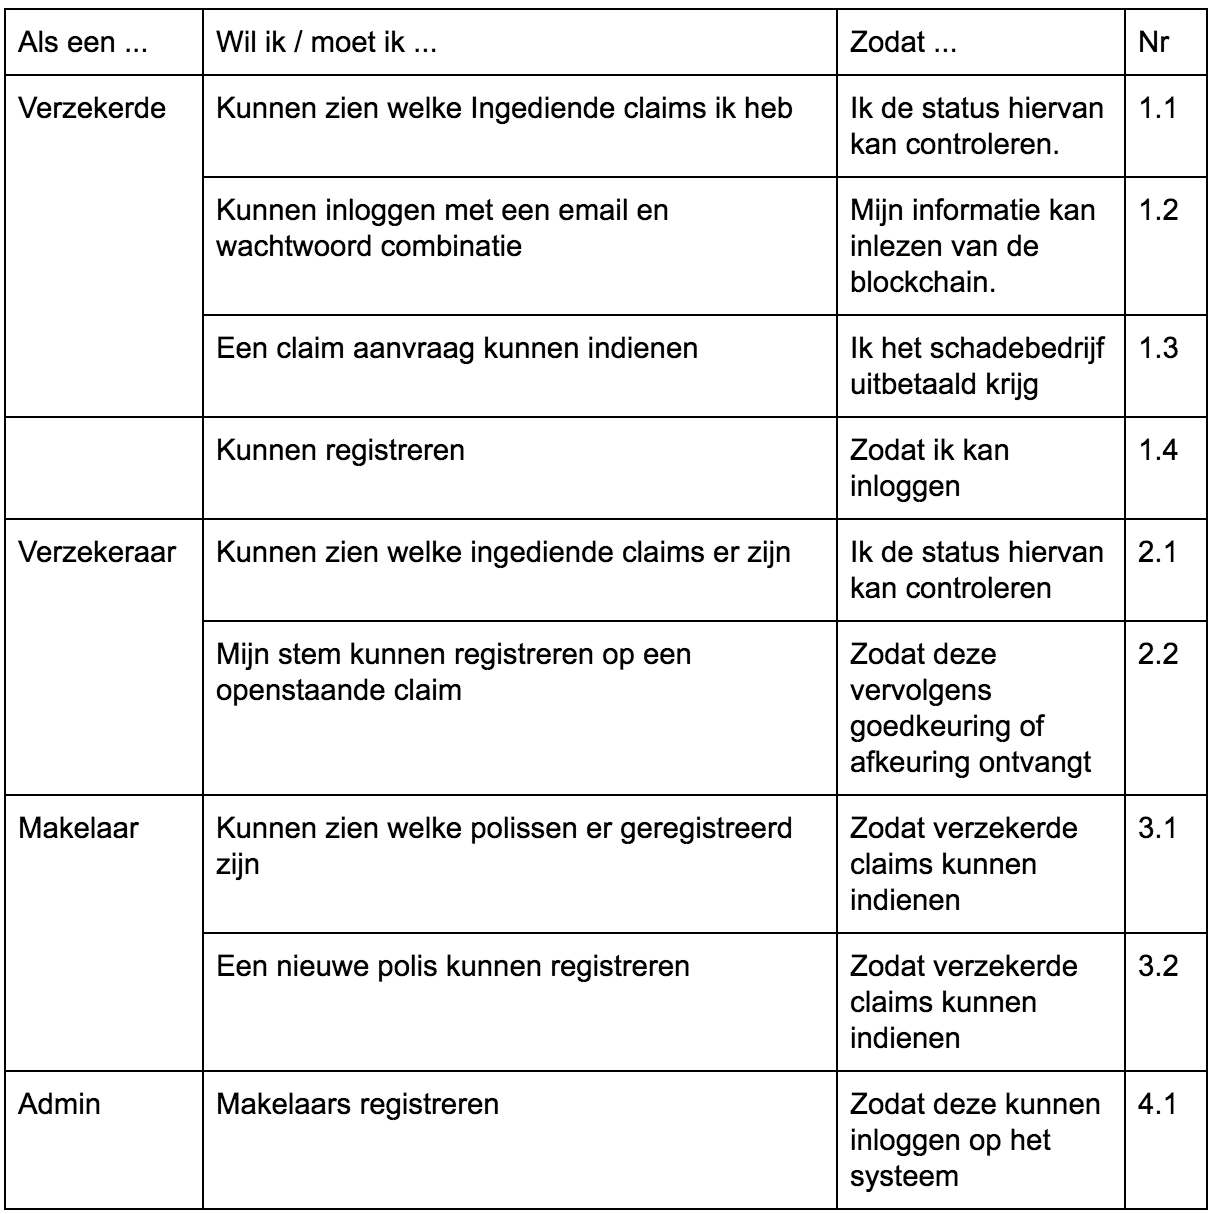
\includegraphics[scale=0.7]{images/userstories}
        \caption{User stories die de functionele requirements defineren en het development van het proof of concept leiden.}
        \label{fig:userstories}
    \end{center}
\end{figure}

\newpage

\begin{figure}[h!]
    \begin{center}
        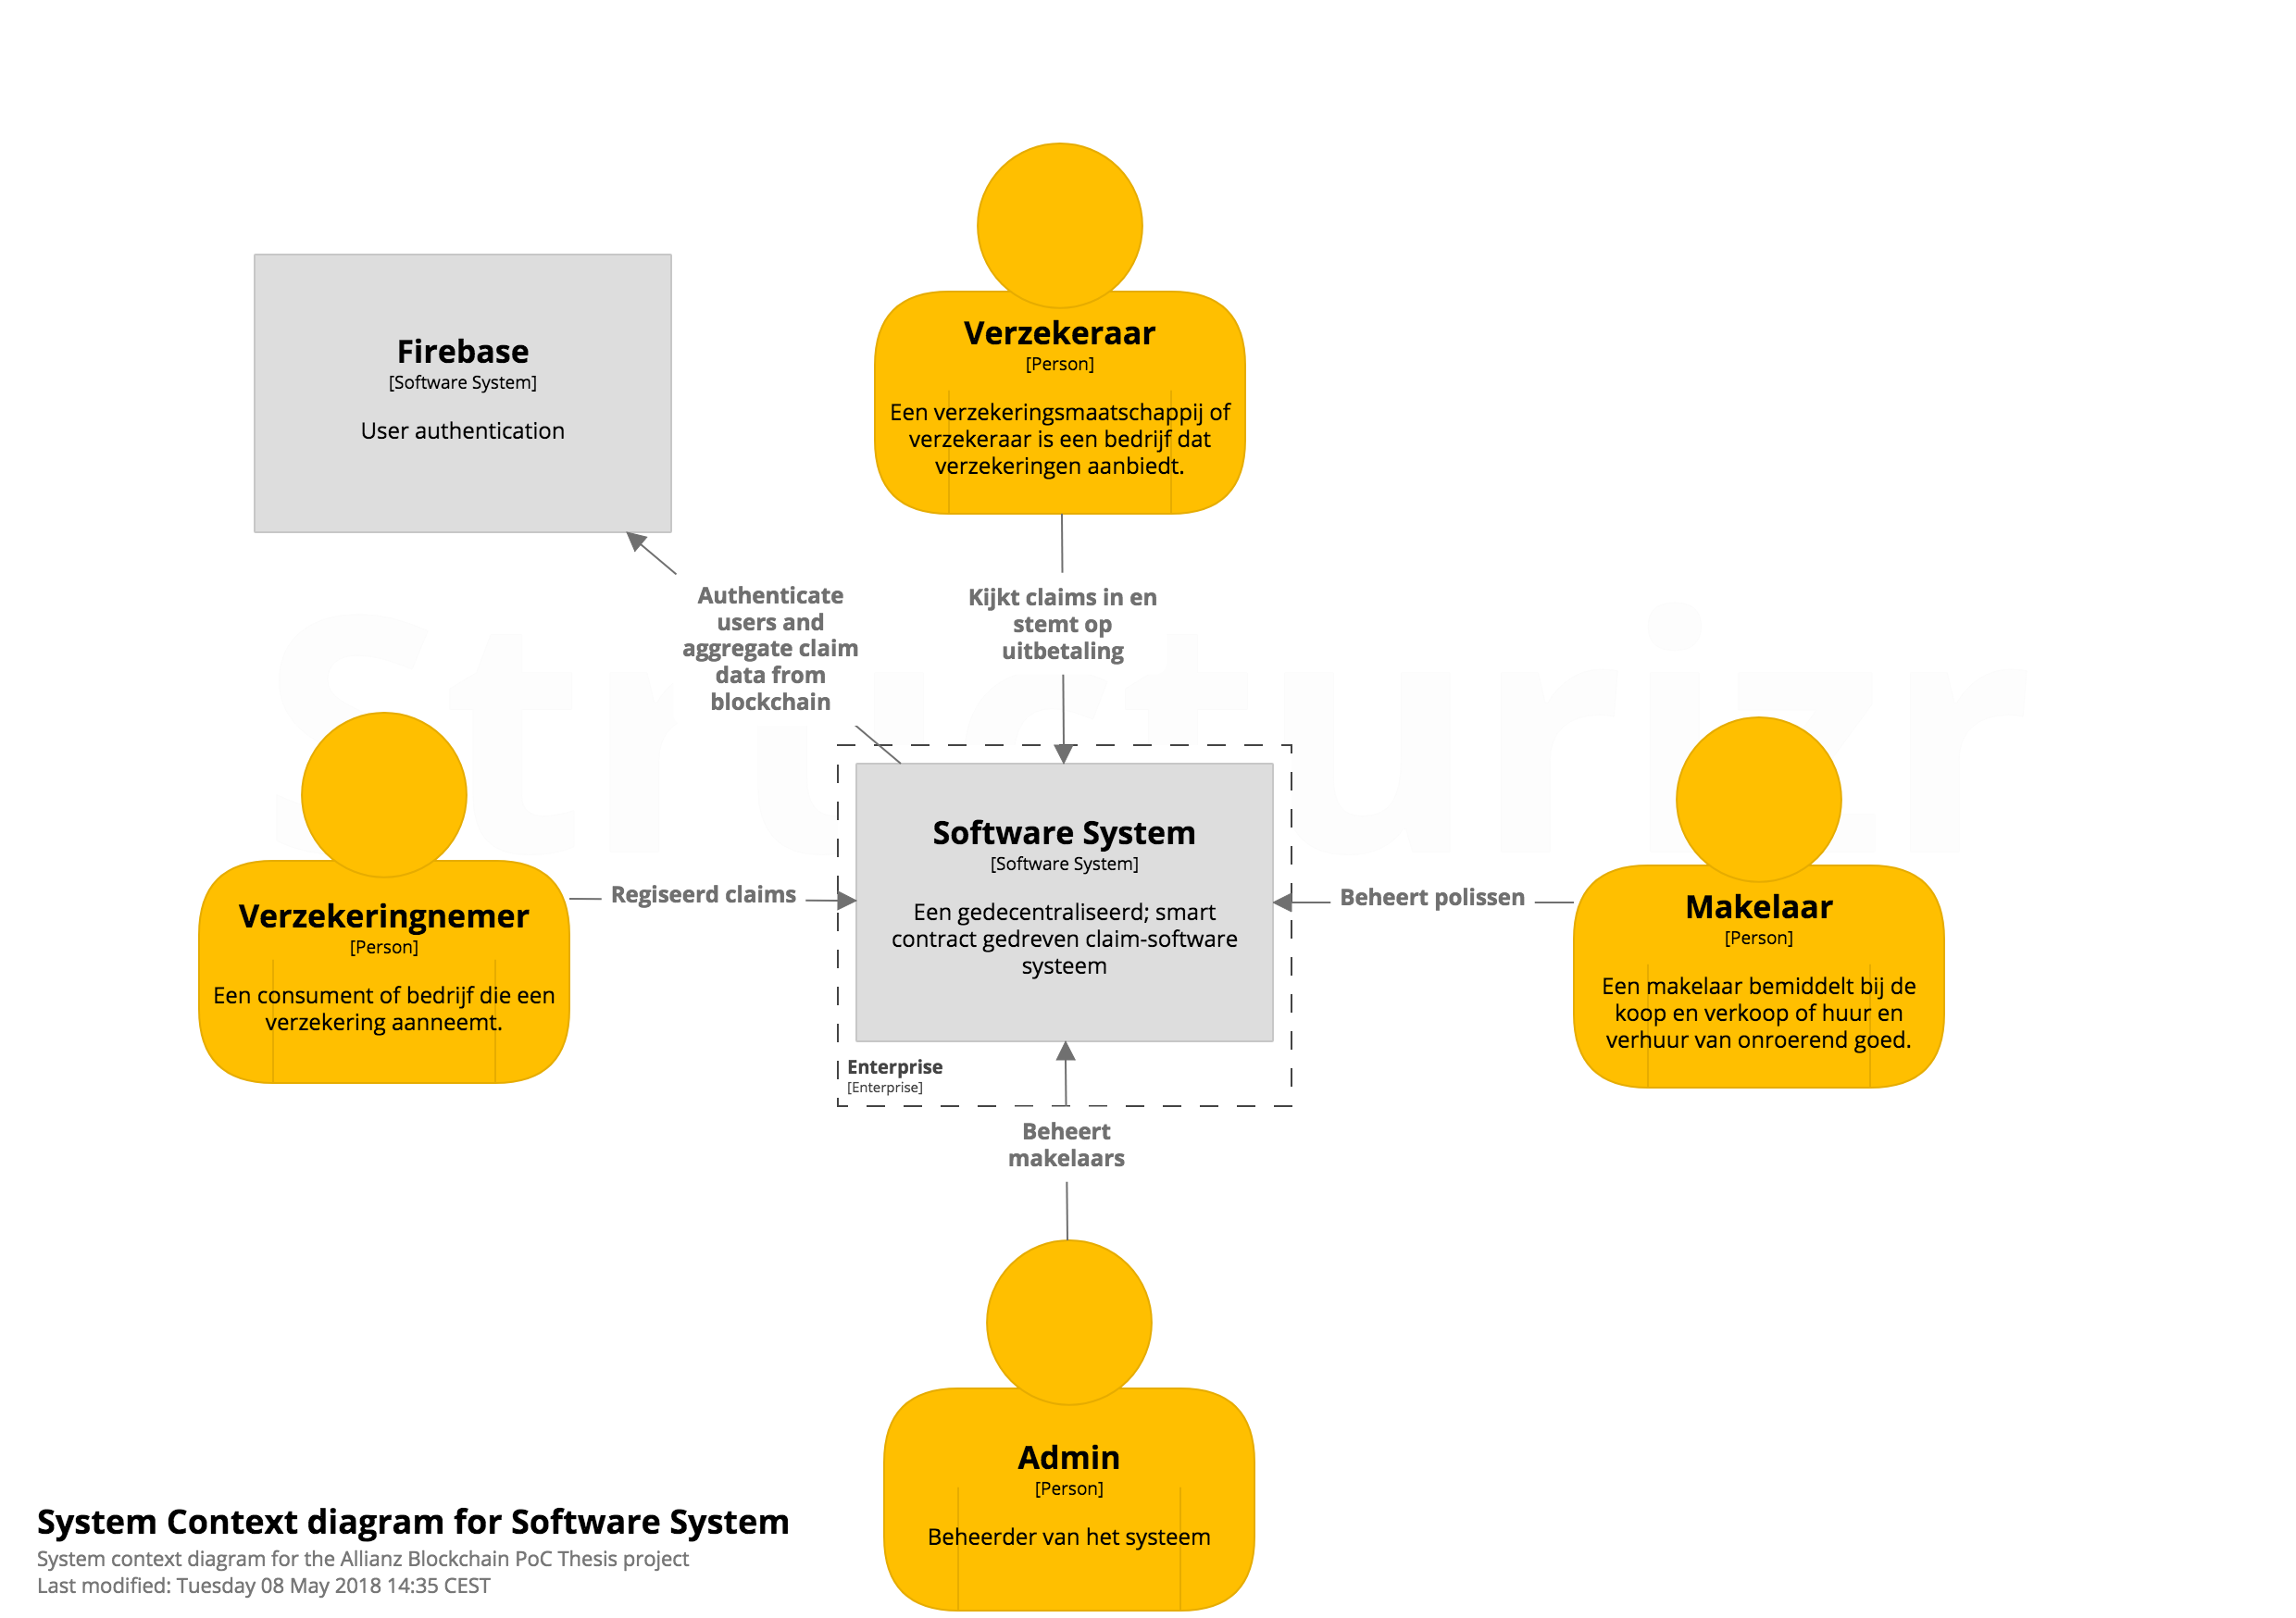
\includegraphics[width=\paperwidth-100]{images/context}
        \caption{C4 - Context.}
        \label{fig:c4Context}
    \end{center}
\end{figure}

Verzekernemers zijn consumenten of bedrijven die een verzekering heeft en met een polisnummer claims kan aanvragen en de status van kan ophalen. De manier waarop gebruikers via de backend interactie hebben met de smart contract in de Ethereum blockchain word getoond in figuur \ref{fig:c4Context}.

\begin{figure}[h!]
    \begin{center}
        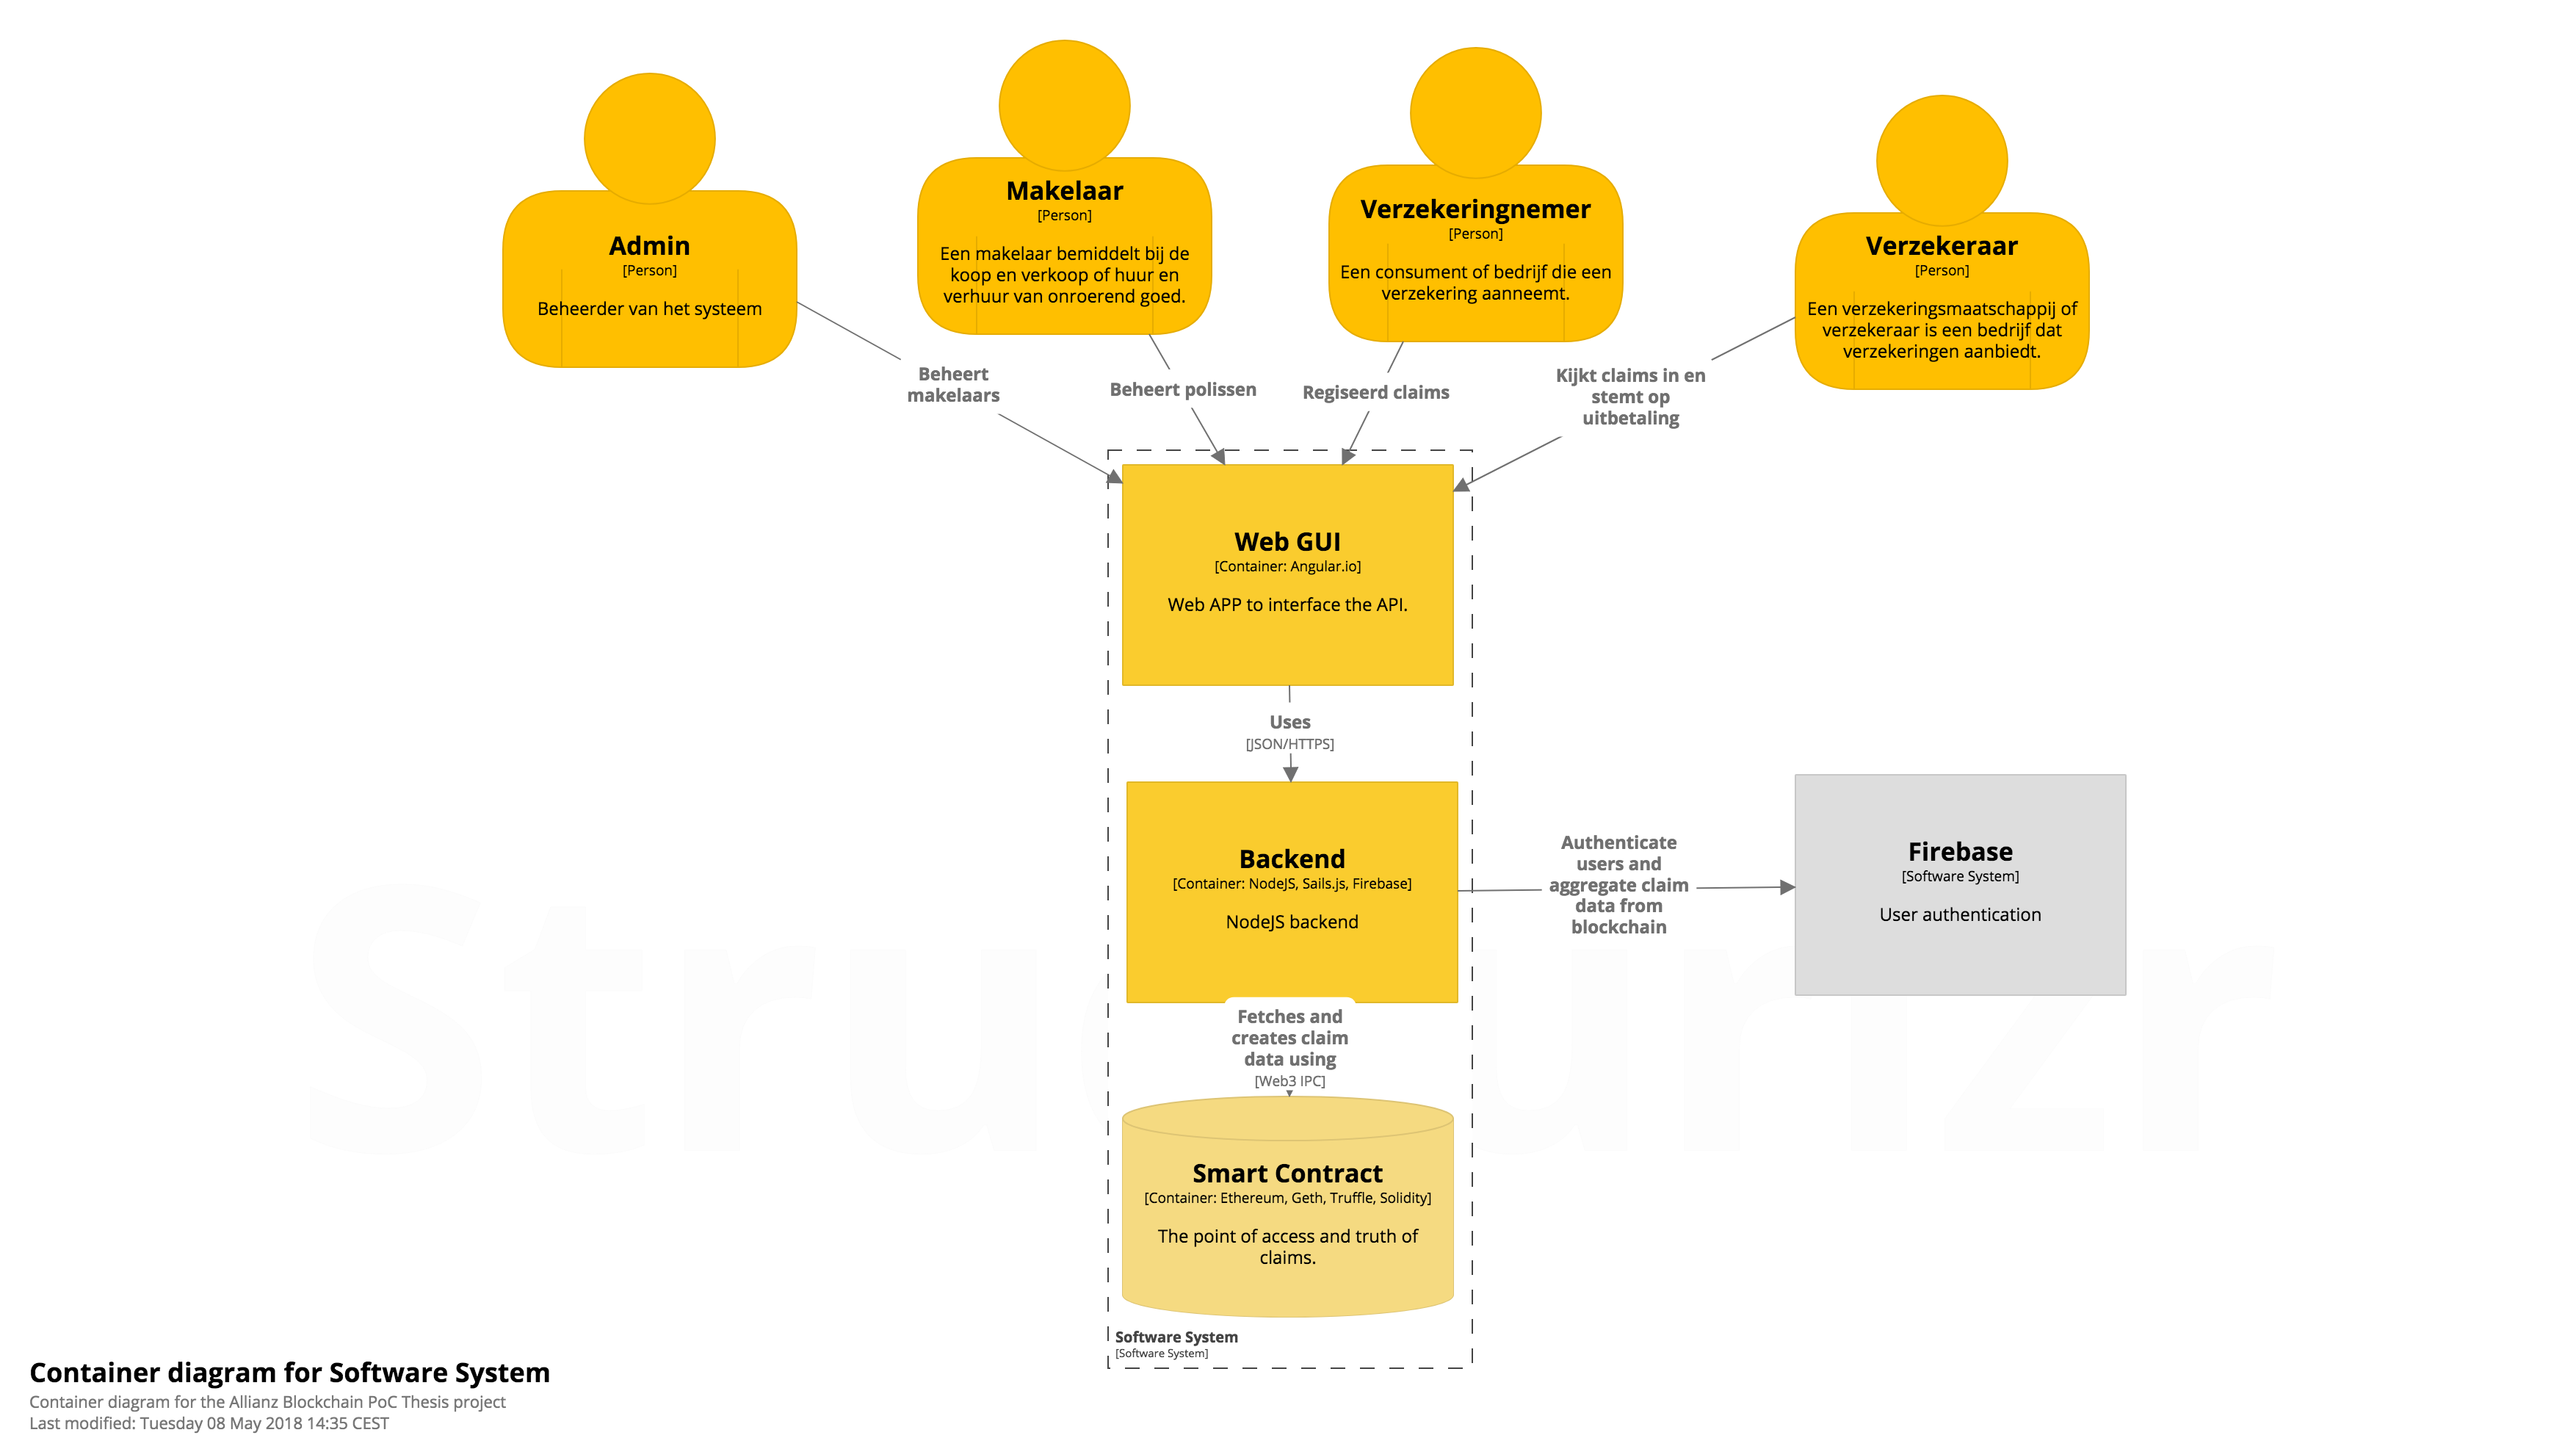
\includegraphics[width=\paperwidth-100]{images/containers}
        \caption{C4 - Containers.}
        \label{fig:c4Containers}
    \end{center}
\end{figure}

In de onderstaande opsomming staan de non-functinoele requirements die ook aan het PoC worden gesteld.
\begin{itemize}
  \item \textbf{R1.} Het systeem geeft gebruikers toegang op basis van hun email en wachtwoord
  \item \textbf{R2.} Het systeem controleert bij een claim aanvraag van of het polis nummer valide is
  \item \textbf{R3.} Het systeem moet automatisch goedkeuring geven voor een claim als het claimbedrag onder 1000 euro zit en het type diefstal is.
  \item \textbf{R4.} Met gebruik van smart contracts en de blockchain wordt de data integriteit gewaarborgd.
  \item \textbf{R5.} Een verzekeraar kan bij het aanmaken van een nieuwe polis aangeven wat de verdeling is tussen de verzekeringsmaatschappijen.
\end{itemize}

The design of the final PoC was based on the requirements and user stories mentioned above.


%%%%%%%%%%%%%%%%%%%%%%%%%%%%%%%%%%%%%%%%%%%%%%%%%%%%%%%%%%%%%%%%%%%%%%%%%%%%%%
%%
%% Bibliography:
%%
%\cleardoublepage
%\phantomsection
\addcontentsline{toc}{chapter}{Bibliografie}
\bibliography{thesis}

% %%%%%%%%%%%%%%%%%%%%%%%%%%%%%%%%%%%%%%%%%%%%%%%%%%%%%%%%%%%%%%%%%%%%%%%%%%%%%%%%
% %% Appendix:
% %%

\chapter{Bijlagen}
\appendix
\chapter{test}\label{chap:test}
cool



%%%%%%%%%%%%%%%%%%%%%%%%%%%%%%%%%%%%%%%%%%%%%%%%%%%%%%%%%%%%%%%%%%%%%%%%%%%%%%%%
%% Index:
%%
% \printthesisindex

\end{document}
